%
% Copyright (c) 2011-2012, fortiss GmbH.
% Licensed under the Apache License, Version 2.0.
% 
% Use, modification and distribution are subject to the terms specified
% in the accompanying license file LICENSE.txt located at the root directory
% of this software distribution. A copy is available at
% http://chromosome.fortiss.org/.
%
% This file is part of CHROMOSOME.
%
% $Id$
%
% Author:
%         Dominik Sojer <sojer@fortiss.org>
%         Michael Geisinger <geisinger@fortiss.org>
%

\documentclass[11pt,twoside,a4paper]{article}
\usepackage[margin=1in]{geometry}
\usepackage{graphicx}
\usepackage{listings}
\usepackage{xspace}
\usepackage{color}
\usepackage[colorlinks=true,urlcolor=blue,citecolor=blue,linkcolor=blue]{hyperref}
\usepackage{units}

\usepackage{fancyhdr}
\setlength{\headheight}{15.2pt}
\fancyhead{}
%\fancyhead[LE,RO]{\rightmark}
\fancyhead[LE,RO]{\leftmark}
\fancyfoot{}
\fancyfoot[C]{\thepage}
\pagestyle{fancy}

\newcommand{\TODO}[1]{{\color{red}{#1}}}
\newcommand{\xme}{\textsf{CHROMOSOME}\xspace}
%\renewcommand{\thesection}{\arabic{section}.}

\lstset{basicstyle=\tt\footnotesize,language=c,tabsize=4,escapechar=\~,emph={Add,Change,Comment,Uncomment,remove,or,this,line,block,Leave,the,rest,of,function,as,is,all,following,lines},emphstyle={\color[rgb]{0,0,0.75}},keywordstyle={\color[rgb]{0,0.5,0}\bfseries},commentstyle={\color[rgb]{0.5,0.5,0.5}\bfseries},stringstyle={\color{red}}}
\let\origthelstnumber\thelstnumber
\makeatletter
\newcommand*\LstSuppressNumber{%
	\lst@AddToHook{OnNewLine}{%
		\let\thelstnumber\relax%
		\advance\c@lstnumber-\@ne\relax%
	}%
}
\lstdefinelanguage{cmake}{%
	morekeywords={xme_link_components,xme_add_component},
	sensitive=false,
	morecomment=[l]\#,
	morestring=[b]",
}
\newcommand*\LstReactivateNumber{%
	\lst@AddToHook{OnNewLine}{%
		\let\thelstnumber\origthelstnumber%
	\advance\c@lstnumber\@ne\relax}%
}

\widowpenalty=1000
\clubpenalty=1000

\title{\textsf{CHROMOSOME in 120 Minutes} \\ 
\includegraphics{figures/PNG/title.png}}
\author{%
	Fortiss GmbH\\[6pt]
	An-Institut der\\
	Technischen Universit\"at M\"unchen\\[6pt]
	Guerickestr. 25\\
	80805 M\"unchen\\[6pt]
	\url{chromosome@fortiss.org}
}
\date{Version 0.2\\April 2, 2012}

\begin{document}
\maketitle

\vfill
\begin{quote}
Copyright (c) 2011-2012, fortiss GmbH.\\
Licensed under the Apache License, Version 2.0.\\[6pt]

Use, modification and distribution are subject to the terms specified
in the accompanying license file LICENSE.txt located at the root directory
of this software distribution. A copy is available at
\url{http://chromosome.fortiss.org/}.
\end{quote}

\newpage
\tableofcontents
\newpage

%
% Copyright (c) 2011-2012, fortiss GmbH.
% Licensed under the Apache License, Version 2.0.
% 
% Use, modification and distribution are subject to the terms specified
% in the accompanying license file LICENSE.txt located at the root directory
% of this software distribution. A copy is available at
% http://chromosome.fortiss.org/.
%
% This file is part of CHROMOSOME.
%
% $Id$
%
% Author:
%         Dominik Sojer <sojer@fortiss.org>
%         Michael Geisinger <geisinger@fortiss.org>
%

\section{Introduction} \label{sec:intro}

For a long time, the focus of embedded systems development has been the implementation of isolated systems with clearly defined borders and interfaces.
Recently, the trend of integrating these complex independent systems into larger \emph{systems of systems} arises:
manufacturing plants get connected with logistics, intelligent cars communicate with each other and the infrastructure. 
Due to the different life cycles of the different involved systems, adaptability in the sense of plug\&play becomes more and more important. Systems must 
be integrated with other systems although the concrete systems were not know at design time. Future embedded systems have to be developed in a way so 
that they can be integrated into these systems of systems without losing their safety, security and real-time capabilities. 

In order to achieve this, a powerful domain-independent software platform is required,
which can flexibly be adapted to various application scenarios.
\xme\footnote{\url{http://chromosome.fortiss.org/}} is a middleware and runtime system intended to meet these requirements. It combines features known
from the embedded domain such as determinism where necessary with adaptivity known from internet technologies. \xme treats extra-functional requirements as 
first-class entity and provides according mechanisms to fulfill the application requirements.

\xme has a large set of designated features and is designed to evolve over time.
It is completely open source and hence transparent to developers and end users.
The current release includes a first subset of the features that will be available in future versions.
Although we have a clear vision of the final system, \xme's development is demand driven.
Its goal is to provide adequate platform support and tooling for maximum efficiency.

The following tutorial will introduce you to the main concepts of \xme and illustrate them with examples that are easy to understand.
Including installation of required prerequisites, this tutorial will take about two hours to complete.

\subsection{The Name \xme}
\xme stands for \textbf{\underbar{Cro}}ss-domain \textbf{\underbar{M}}odular
\textbf{\underbar{O}}perating \textbf{\underbar{S}}ystem \textbf{\underbar{o}}r
\textbf{\underbar{M}}iddlewar\textbf{\underbar{e}}.
The name expresses the vision of \xme:
\begin{enumerate}
	\item We believe that in the future cross-domain solutions will be required.
	\item As different applications might have many different requirements
		and the middleware will be deployed to very heterogeneous platforms,
		a scalable and modular solution is required.
	\item \xme will sometimes operate on top of an operating system (OS),
		but it might also replace an OS due to resource reasons.
		Therefore, we think that in the future,
		the boundary between an operating system and a middleware might get blurred.
\end{enumerate}

Similar to biology, a \xme instance can be built up a number of genes (modules).
It is not the intention of \xme to invent new genes, but instead to use
existing protocols / solutions to implement components for specific tasks.
The major idea is that \xme offers a flexible blueprint that enables the
selection of different solutions to adapt a system to the specific requirements.

Analog to the evolution of mankind, we do not believe that the genes,
but also the blueprint provided by \xme are initialy perfect.
Instead we believe in constant improvement based on discussions about specific components.
This is one of the reasons why we are offering \xme as open-source software.
In case you have any questions or suggestions for improvement, we are looking forward to your comments.

\subsection{Questions and Contact Information}

If you have any questions with respect to this tutorial or want to report a bug,
please check the Frequently Asked Questions in Appendix~\ref{appx:faq}.
If your question is not answered, please do not hesitate to send an e-mail to \url{chromosome@fortiss.org}. Thank you!

\subsection{Acknowledgements}

This work is partially funded by the following research grants:
\begin{itemize}
	\item German Federal Ministry of Economics and Technology (BMWi) research grant 01ME12009
		(project RACE\footnote{\url{http://www.projekt-race.de/}})
	\item German Federal Ministry of Economics and Technology (BMWi) research grant 01MA11002
		(project AutoPnP\footnote{\url{http://www.autopnp.com/}})
	\item Bavarian Ministry of Economic Affairs, Infrastructure, Transport and Technology grant programme 1330/686
		(Vorlaufforschung Fortiss)
\end{itemize}
\clearpage
%
% Copyright (c) 2011-2012, fortiss GmbH.
% Licensed under the Apache License, Version 2.0.
% 
% Use, modification and distribution are subject to the terms specified
% in the accompanying license file LICENSE.txt located at the root directory
% of this software distribution. A copy is available at
% http://chromosome.fortiss.org/.
%
% This file is part of CHROMOSOME.
%
% $Id$
%
% Author:
%         Dominik Sojer <sojer@fortiss.org>
%         Michael Geisinger <geisinger@fortiss.org>
%

\section{Prerequisites (20 minutes)}
\xme has been developed with platform independence in mind, but for sake of simplicity,
this tutorial uses a Windows-based development environment and a Windows-based target platform.
%
While installing the proposed build environment, you might want to start reading Section~\ref{sec:architecture} giving an overview on \xme and its features.

Apart from the \xme source archive, two tools are recommended for building \xme applications on Windows.
\begin{itemize}
	\item \textbf{Visual Studio C++} (Express, Professional, Premium or Ultimate, preferably 2008 or 2010 versions):
		Visual Studio is Microsoft's platform for multi-language development.
		The so-called ``Express Edition'' is available free for evaluation purposes\footnote{%
		\url{http://www.microsoft.com/visualstudio/en-us/products/2010-editions/visual-cpp-express}}.
		Note that \xme has not yet been tested with Visual Studio 2011, of which a beta version has been recently released.
		You only have to install the C/C++ compiler, Additional packages like Silverlight or SQL Server are not required.
		Consult Appendix~\ref{appx:install_vs} for details.
	
	\item \textbf{CMake} (at least version 2.8.5):
		CMake is a cross-platform Makefile generator and is used to manage the build system.
		%Input to CMake are a set of \texttt{CMakeLists.txt} files that contain the specifications for the build system.
		Output of CMake are the build system configurations (e.g., a UNIX Makefile, a Microsoft Visual Studio Project, an Eclipse CDT project).
		\xme provides a customized set of macros to deal with components, dependencies, executables and documentation.
		CMake can be downloaded for free\footnote{\url{http://www.cmake.org/cmake/resources/software.html}}.
		\xme currently requires at least CMake version 2.8.5.
		It is \emph{not} necessary to add CMake to the system search path.
		Consult Appendix~\ref{appx:install_cmake} for details.
\end{itemize}

\clearpage
%
% Copyright (c) 2011-2012, fortiss GmbH.
% Licensed under the Apache License, Version 2.0.
% 
% Use, modification and distribution are subject to the terms specified
% in the accompanying license file LICENSE.txt located at the root directory
% of this software distribution. A copy is available at
% http://chromosome.fortiss.org/.
%
% This file is part of CHROMOSOME.
%
% $Id$
%
% Author:
%         Dominik Sojer <sojer@fortiss.org>
%         Michael Geisinger <geisinger@fortiss.org>
%

\section{\xme in a Nutshell (30 minutes)} \label{sec:architecture}

\xme (often abbreviated by ``XME'') is a domain-independent, data-centric\footnote{%
For details, please refer to \url{http://www.omg.org/news/whitepapers/Intro_To_DDS.pdf}}
middleware for cyber-physical systems.
%
From the point of view of an application component,
\xme abstracts from basic functionality that is traditionally found in operating systems and middlewares,
like scheduling and communication.
%
This section will give the reader a very high level overview of the most important \xme features.
For in-depth information and concrete specifications, the reader is kindly referred to the commented source code of \xme.

\subsection{Goals of \xme}
\xme is designed to match the requirements of future cyber-physical systems.
As a research prototype, the main intention is to serve as a basis
for discussion how future middleware/operating system architectures may look like.
The development is done in a demand-driven way.
Depending on the requirements of projects where \xme is applied, new features in \xme will be introduced.

The current version is the first version of \xme and therefore provides only very basic funcitonality.
Further features will be introduced in the future. In the following, the main concepts of \xme are introduced.
In addition, we state whether these features are already implemented or planned for future versions.
%In the following, the goals of \xme and major concepts to achieve these goals are listed.
%
%\subsubsection{Scalability \& Modularity}
%
Our point of view is that
future middleware will not operate on a specific class of devices, but will run on very heterogeneous platforms.
The exaggerated goal statement could be to ``develop a middleware serving a range from 8-bit controllers to cloud servers''.

Therefore, scalability and modularity of the middleware is of highest importance. It must be easy to remove or add components from/to 
the middleware. Similar to micro-kernel operating systems, the core of \xme must be very small and only contain the absolutely necessary
features. Since the boundaries of operating systems, middleware, and applications are vanishing, one unique mechanism must be supported to
add components on all these levels.

\paragraph{Concept 1: Data-Centric Design} A very succesful concept to achieve scalability is message-orientation as for example demonstrated
by the QNX\footnote{\url{http://www.qnx.com/}} neutrino micro-kernel.
However, one major drawback of this concept is the necessity of requiring knowledge of both the sender and the receiver.
In the context of systems-of-systems where the communication partners are not known at design time, message orientation cannot be applied.
Therefore, \xme is based on the very powerful concept of data-centric design. Components specify which data they consume
and produce and based on this information, the middleware calculates the communication routes.

It is important to note that in contrast to prominent other middleware systems relying on data-centric design,
\xme does not broadcast the data, instead it calculates specific routes based on the requirements.
This allows for a very efficient implementation. Furthermore, the routes are calculated only when components are added or removed. Based
on the experience in embedded systems, we assume that reconfiguration takes places less often than the transmission of data items.
Similar to concepts from multimedia protocols,
our initial assumption is that data transmission has to happen within real-time,
while reconfiguration is not time-critical or has only soft real-time requirements.

Data is grouped by so-called \emph{topics}. A topic is a data type with a certain structure.
Examples for topics are temperature or rotation speed. Topics are defined for a specific domain.
This enables the exchange of data between different applications.
To allow cross-domain communication, we plan to define translation matrixes between the topics of different domains.

\paragraph{Concept 2: Meta-Data Support (not yet implemented)}
	Exchange of data can only be automated if the requirements on data are specified explicitly.
	This includes information about the quality of data such as age, accuracy, confidence, and safety level.
	In the future, we plan to support respective annotations to data, so-called \emph{meta-data}, to specify these requirements.
	
	Using meta-data, application components describe their requirements respectively guarantees on data.
	This information can be used to select appropriate communication streams while still retaining independence between sender and receiver.
	
	We are planning to support two scenarios:
	\begin{itemize}
		\item \textbf{Static meta-data:}
			Application components have fixed requirements and guarantees.
			Meta-data are used to calculate the appropriate communication routes at configuration time.
			For example, imagine a temperature sensor network for building automation.
			Depending on its size, multiple sensors may be present in a room.
			Each sensor would specify its \emph{location} as meta-data.
			A climate control component that controls the air conditioning system for a specific room would specify, using meta-data,
			that it only wants to receive temperature data from sensors that match the respective room.
		
		\item \textbf{Dynamic meta-data:}
			Application components producing data may specify meta-data such as the quality of the transmitted values dynamically during runtime.
			Consuming components may have dynamic meta-data acceptance filters and may use meta-data also for their calculations.
			For example, imagine that one of the rooms in the auotmated building from the previous example is a server room.
			In this case, a high reliability is required.
			Using meta-data about the confidence of each sensor,
			the climate control may dynamically calculate the confidence in its own set value for the air conditioning system.
			The association of data from the respective room could still use static meta-data.
	\end{itemize}

\paragraph{Concept 3: Data Access}
Components can access data in two different ways. As standard operation, \xme provides a publish-subscribe mechanism. Each component states
which data is required and which data is produced. The middleware ensures the routing of the specific data. If data is only required 
seldomly in comparison to the data production rate, a request-response mechanism is offered to the application developer.

\paragraph{Concept 4: Timing (not yet implemented)}
Correct timing is a major concern for cyber-physical systems. \xme abstracts the concrete implementation, but will offer mechanisms to
specify end-to-end-timing and jitter requirements for data paths.
The reason to abstract the concrete implementation / concrete configuration
in \xme is on the one hand to reduce the development effort by automatically deriving a concrete configuration satisfying the timing
requirements (if a configuration exists) and on the other hand to support plug~\&~play capability. The state of the art in embedded system
design requires the developer to configure the application in a correct way. Several configurations might be valid, but typically only one
configuration is specified. It is not possible for the run-time system to change the configuration, as the real requirements are not present
any more and the system can not calculate alternative configurations. By explicitly stating the requirements and leaving configuration issues
to the run-time system, this problem can be avoided.
The system can support new components by calculating a new configuration that satisfies both
the requirements of already running applications and the newly installed applications.

It is important to note that \xme can of course only offer guarantees that are enabled by the underlying platform.
In case \xme runs on Windows, \xme will not be able to satisfy jitter requirements in the range of microseconds.
Nevertheless, different implementations of components will offer very good guarantees.
The major concept here is to use algorithms that offer determinism sacrificing average-case performance.
Examples are the implementation of a time-triggered communication scheme on top of Ethernet.
This implementation guarantees collision free communication, but comes with a lower bandwidth and flexibility.

\paragraph{Concept 5: Resource-Awareness (not yet implemented)}
\xme is designed to be able to handle all resources of the platform.
The major idea is that components / applications can state their worst-case resource requirements
on memory, computation time, bandwidth, etc.
\xme will then ensure that enough resources are available to allow the execution of this component / application.

\paragraph{Concept 6: Other extra-functional properties -- Fault-tolerance, QoS, Security (not yet implemented)}
\xme is designed in a way such that components which guarantee other extra-functional properties can be easily extended.
Examples on extra-functional properties that are currently being integrated in \xme are fault-tolerance, QoS, and security.

\paragraph{Concept 7: Support for States (not yet implemented)}
A very important topic to ensure resource efficiency is state awareness.
We are currently thinking about possibilities to support states
(each one with a set of active applications) in \xme.
The support of (sub-)system wide states would simplify the development of applications,
but also other aspects such as fault-tolerance.

\begin{figure}[htb]
	\centering
	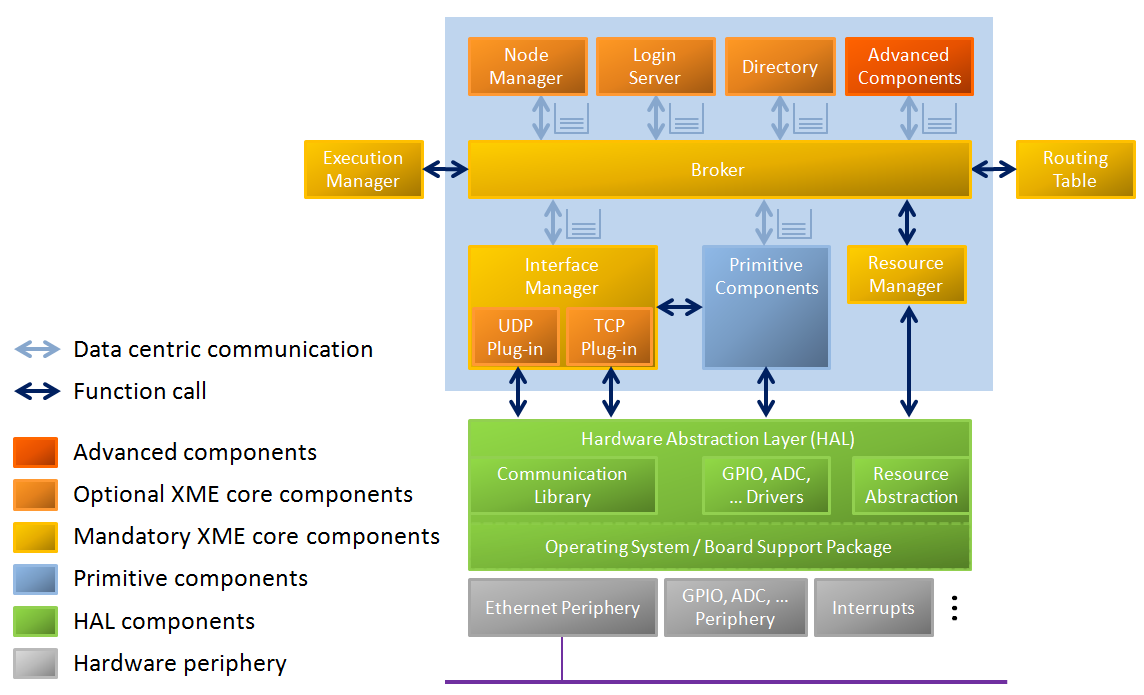
\includegraphics[width=\textwidth]{figures/PNG/architecture.png}
	\caption{\xme architecture overview.}
	\label{fig:architecture}
\end{figure}

\subsection{Core Components}
\label{sec:core_components}
\xme is designed in a modular fashion. Its component-oriented architecture is depicted in Figure~\ref{fig:architecture}.
A (distributed) \emph{application} consists of a set of (software) \emph{components} that interact with each other by exchanging data.
Each component is placed on a specific \emph{node} in the network.
On operating system based platforms like Windows,
the software of a node is typically represented by a console application.
On embedded systems, the software of a node corresponds to the firmware.
%
The following sections provide brief descriptions of the most important core components of \xme.
See Figure~\ref{fig:architecture} for a graphical illustration.

\subsubsection{Node Manager}

A node can have an arbitrary amount of software components that implement the application.
The \emph{Node Manager} is responsible for connecting a new node to the network and obtaining a so-called \emph{node identifier}.
The node identifier is a unique address of the node within a network.
The Node Manager periodically tries to obtain such a node identifier from the \emph{Login Server},
which is present on one specific node in the network.

\subsubsection{Login Server}

The \emph{Login Server} maintains a list of all nodes in the \xme network.
It receives login requests from the Node Managers of all other nodes and handles them accordingly.
Only one Login Server should exist in the network.

\subsubsection{Directory}

The \emph{Directory} maintains a list (a directory, as the name implies)
of all publication and subscription requests in the network
and is responsible for root calculation and setup.
Usually, only one so-called \emph{Master} Directory exists in the network, which is the autority for route calculation.
All other nodes have a so-called \emph{Local} Directory, which is only authoritative for local routes
and forwards announcements (publication and subscription requests) to the Master Directory.
Setup of routes is performed by modifying the \emph{Routing Tables} present on every node.

\subsubsection{Routing Table}

As the name implies, the \emph{Routing Table} is a data structure that contains routing information.
In \xme, routing is performed via so-called \emph{data channels}.
A data channel is a system-internal identifier for a communication path.
When data arrive at a node, the Routing Table is inspected to determine where the data has to be delivered to.
This is done by the \emph{Broker}.

\subsubsection{Broker}

The \emph{Broker} is response for delivering incoming data to the correct destination,
which can be determined from the Routing Table.
The Broker is also responsible for buffering the data if it can not be delivered immediately.
The decision of when data can be delivered to a component is issued by the \textit{Execution Manager}.

\subsubsection{Execution Manager}

The \emph{Execution Manager} is the facility that enforces the model of execution in the system
(according to a schedule).
It determines when tasks are executed and when incoming data are processed by components.
Data that are not immediately processed are put into queues.

\subsubsection{Resource Manager}

The \emph{Resource Manager} is the node-local authority for resource reservation and arbitration.
Among others, managed resources include memory and CPU time.
Components report their requirements to the directory and only get them assigned when enough resources are available.

\subsubsection{Interface Manager}

The \emph{Interface Manager} abstracts from the communication interfaces available at a certain node.
Typical submodules of the Interface Manager are facilities for communication over Ethernet/IP with UDP or TCP.
When data is to be sent, it is delivered from the Broker to the Interface Manager.
Incoming data from the network is forwarded to the Broker to decide where to deliver it to.

\subsubsection{Primitive Components}

\emph{Primitive Components} directly access the \emph{Hardware Abstract Layer} using function calls
and offer data obtained from the hardware in a data centric way or forward data to the respective actuators.
They are typically the source of physical data obtained from the environment and
the sink for control data to the environment.

\subsubsection{Hardware Abstraction Layer}

The \emph{Hardware Abstraction Layer}, often abbreviated by HAL,
provides a platform indepdent application programming interface (API).
\xme components are implemented against that API and hence are platform independent.
The HAL typically implements hardware-specific functionality such as drivers for microcontroller periphery
like general purpose I/O (GPIO) or analog to digital conversion (ADC).

\subsubsection{Advanced Components}

The actual (distributed) application running in the network is implemented by application-specific \emph{Advanced Components}.
Advanced Components operate solely on data obtained via data centric communication.
In particular, no direct access to the Hardware Abstraction Layer with effects in the environment is allowed.

\subsubsection{Login Client Proxy and IP Login Server Proxy}

These components are required for new nodes to initially contact the Login Server.
A node that does not have a Login Server will usually have a \emph{Login Server Proxy} component for each of its physical network interfaces.
These components are named according to their associated interface types,
for example \emph{IP Login Server Proxy} for an Ethernet interface with IP communication stack.
Whenever the Node Manager, which is responsible for periodic login requests, issues a login request,
the Login Server Proxy takes care of broadcasting it over its associated communication interface.

Nodes that have a Login Server component usually also have a \emph{Login Client Proxy} for each of their interfaces.
The Login Client Proxy will receive the login requests issued by the Login Server Proxy on the respective medium
and forward them locally to the Login Server.
The login response is forwarded in a similar manner.
%
This concept makes it possible to separate the login and address assignment logic from specific interface types and communication protocols
and enables a fine-grained assignment of functionality to each communication interface.

\subsection{Component Definition and Lifecycle}
\label{sec:component_definition}

\xme components are assigned to one of the following categories according to their ``layer'' within the system:
\verb|adv| (advanced), \verb|prim| (primitive), \verb|core| (runtime system) or \verb|hal| (hardware abstraction).
A \xme component is defined by four functions to \emph{create}, \emph{activate}, \emph{deactivate} and \emph{destroy} it,
illustrated here for a component called \verb|xme_adv_myComponent|:
\begin{quote}
	%\verb|xme_core_status_t|\\
	\verb|xme_adv_myComponent_create(xme_adv_myComponent_configStruct_t*);|\\
	%\verb|xme_core_status_t|\\
	\verb|xme_adv_myComponent_activate(xme_adv_myComponent_configStruct_t*);|\\
	%\verb|void|\\
	\verb|xme_adv_myComponent_deactivate(xme_adv_myComponent_configStruct_t*);|\\
	%\verb|void|\\
	\verb|xme_adv_myComponent_destroy(xme_adv_myComponent_configStruct_t*);|
\end{quote}
%
The distinction between creation/activation and deactivation/destruction is required in case a component needs to be migrated:
in this case, the component is first deactivated (to obtain a consistent state), then moved and activated at the new location.
All four functions take a pointer to a configuration structure, which represents the state of the respective component instance.
Multiple component instances of the same component type usually have their own configuration structures.

A typical task during creation of a component is registration of data demand and data production.
Furthermore, a component may create (periodic) tasks to implement its functionality.
These two concepts are illustrated in the following sections.

\subsection{Component Instantiation}

Components can be instantiated by adding them to the so-called \emph{component list}, usually defined in the main program file.
Mandatory core components (compare Figure~\ref{fig:architecture}) are implicitly added to the list.
An initial configuration may be provided for each component.
Listing~\ref{lst:component_list} shows a sample component list with respective configurations.

\begin{lstlisting}[numbers=left,float=htpb,label=lst:component_list,caption=Sample component list with component configurations.]
/*****************************************************************************/
/***   Component configurations                                            ***/
/*****************************************************************************/
XME_COMPONENT_CONFIG_INSTANCE(xme_core_nodeManager) = ~\label{lst:component_list.initialized_config_begin}~
{
	0x00000000021041A1, // deviceType
	XME_CORE_DEVICE_GUID_RANDOM // deviceGuid
}; ~\label{lst:component_list.initialized_config_end}~

XME_COMPONENT_CONFIG_INSTANCE(xme_prim_ipLoginServerProxy, 1); ~\label{lst:component_list.uninitialized_config}~

/*****************************************************************************/
/***   Component descriptor                                                ***/
/*****************************************************************************/
XME_COMPONENT_LIST_BEGIN
	XME_COMPONENT_LIST_ITEM(xme_core_nodeManager, 0) ~\label{lst:component_list.stateful_1}~
	XME_COMPONENT_LIST_ITEM(xme_prim_ipLoginServerProxy, 0) ~\label{lst:component_list.stateful_2}~
	XME_COMPONENT_LIST_ITEM_NO_CONFIG(xme_adv_myComponent) ~\label{lst:component_list.stateless}~
XME_COMPONENT_LIST_END;
\end{lstlisting}

This example declares that three components (besides internal core components),
namely \verb|xme_core_nodeManager|, \verb|xme_prim_ipLoginServerProxy| and \verb|xme_adv_myComponent|,
will be present on this node.
We can distinguish between the following types of components:
\begin{enumerate}
	\item \textbf{Components with internal state:}
		The \verb|XME_COMPONENT_LIST_ITEM()| macro is used to declare such a component
		(compare lines~\ref{lst:component_list.stateful_1} and~\ref{lst:component_list.stateful_2}).
		The second parameter of the macro is the zero-based index of the respective configuration
		(defined above the list) that is used to initialize the component.
		
		Some components expect some of their configuration variables to be initialized properly.
		For example, the \emph{Node Manager} expects its \emph{device type} and \emph{device GUID}
		members to be set up.
		This is achived by assigning values to the respective members
		when declaring the configuration structure with the \verb|XME_COMPONENT_CONFIG_INSTANCE| macro
		(compare lines~\ref{lst:component_list.initialized_config_begin}--\ref{lst:component_list.initialized_config_end}).
		Configurations for multiple components of the same type can be declared
		by separating multiple initialization blocks with commas and using the respective index in the
		\verb|XME_COMPONENT_LIST_ITEM()| macro.
		
		Other components, like the \emph{IP Login Server Proxy}, do not require any special configuration.
		They only need a properly defined configuration structure to store their state during runtime.
		Again, the \verb|XME_COMPONENT_CONFIG_INSTANCE| macro is used
		with the second parameter set to the number of configuration structures for that component type to create
		(we could also declare multiple components of the same type), in this case one
		(line~\ref{lst:component_list.uninitialized_config}).
	
	\item \textbf{Components without internal state:}
		The \verb|XME_COMPONENT_LIST_ITEM_NO_CONFIG()| macro is used to declare such a component
		(compare line~\ref{lst:component_list.stateless}).
		In this case, \verb|NULL| will be passed in the \verb|config| parameters of the four functions introduced in Section~\ref{sec:component_definition}.
\end{enumerate}

The list item macro calls have to be embedded between the \verb|XME_COMPONENT_LIST_BEGIN| and \verb|XME_COMPONENT_LIST_END| macro calls.
%
Components declared in this list are automatically created and activated during startup
and deactivated and destroyed during shutdown.

\subsection{Sending and Receiving Data}

Before sending data, a component states its intent to the runtime system.
This is necessary to allow the appropriate communication routes to be set up
and is usually performed from within a component's \emph{create} function.
%
For using data centric communication, \verb|#include| the file \verb|"xme/core/dcc.h"|.
%
To inform \xme that a component intends to send data under a specific \verb|topic|, call:
\begin{quote}
	\verb|publicationHandle =|\\
	\verb|    xme_core_dcc_publishTopic(|\\
	\verb|        topic, XME_CORE_MD_EMPTY_META_DATA, NULL|\\
	\verb|    );|
\end{quote}

The actual sending of \verb|data| is performed with:
\begin{quote}
	\verb|xme_core_dcc_sendTopicData(|\\
	\verb|    publicationHandle, &data, sizeof(data)|\\
	\verb|);|
\end{quote}

A component can subscribe to a certain \verb|topic| with a given \verb|receiveTopicCallback| function by calling:
\begin{quote}
	\verb|subscriptionHandle =|\\
	\verb|    xme_core_dcc_subscribeTopic(|\\
	\verb|        topic, XME_CORE_MD_EMPTY_META_DATA, receiveTopicCallback, NULL|\\
	\verb|    );|
\end{quote}
Whenever data matching the given topic is received, the given callback function is invoked.
The last parameter of the function can be used to pass user-defined data to the callback function,
for example a pointer to the component's configuration structure.
%
\verb|receiveTopicCallback| must have a signature matching \verb|xme_core_dcc_receiveTopicCallback_t|, namely:
\begin{quote}
	\verb|void receiveTopicCallback(xme_hal_sharedPtr_t dataHandle, void* userData);|
\end{quote}
\verb|dataHandle| is a reference to the memory where the received data is located.

\subsection{Working with Tasks}

Tasks are allocated via the resource manager,
hence \verb|#include| \verb|"xme/core/resourceManager.h"| to use them.
A component can create one or multiple asynchronous tasks by calling

\begin{quote}
	\verb|taskHandle = |\\
	\verb|    xme_core_resourceManager_scheduleTask(|\\
	\verb|        startMs, periodMs, XME_HAL_SCHED_PRIORITY_NORMAL,|\\
	\verb|        taskCallback, NULL|\\
	\verb|    );|
\end{quote}

This function registers the \verb|taskCallback| function to be scheduled for execution
according to \verb|startMs| (number of milliseconds before first invocation) and
\verb|periodMs| (interval between invocations).
%
The last parameter of the function can be used to pass user-defined data to the callback function,
for example a pointer to the component's configuration structure.
%
\verb|taskCallback| must have a signature matching \verb|xme_hal_sched_taskCallback_t|, namely:
\begin{quote}
	\verb|void taskCallback(void* userData);|
\end{quote}

A task can be suspended or resumed by calling:

\begin{quote}
	\verb|xme_hal_sched_setTaskExecutionState(|\\
	\verb|    taskHandle, <flag>|\\
	\verb|);|
\end{quote}

\verb|<flag>| is a Boolean flag that indicates the new task execution state.
The call will block until the new state can be enforced,
which is not the case while the task's callback function is executed.
%A task's callback function should return periodically
%and the \verb|periodMs| argument in the \verb|xme_core_resourceManager_scheduleTask()| call
%should be used to reschedule themselves at the appropriate points in time.
%
A task can be aborted by calling:

\begin{quote}
	\verb|xme_core_resourceManager_killTask(|\\
	\verb|    taskHandle|\\
	\verb|);|
\end{quote}

If this function is called from the task to kill itself, then it will mark the task for deletion and return immediately.
If it is called from a different task, the function blocks until the task has been removed.
Similarly to suspension and resuming, a task is not removed until its callback function has returned.

\clearpage
%
% Copyright (c) 2011-2012, fortiss GmbH.
% Licensed under the Apache License, Version 2.0.
% 
% Use, modification and distribution are subject to the terms specified
% in the accompanying license file LICENSE.txt located at the root directory
% of this software distribution. A copy is available at
% http://chromosome.fortiss.org/.
%
% This file is part of CHROMOSOME.
%
% $Id$
%
% Author:
%         Dominik Sojer <sojer@fortiss.org>
%         Michael Geisinger <geisinger@fortiss.org>
%

\section{Example 1: Hello World! (20 minutes)}
\label{sec:example_helloworld}

Two steps are required to build an application based on \xme:
the build system has to be generated using CMake and the application needs to be compiled to binary code.
%In \xme, a different build system tree is generated for every single target node in the network.
%This tutorial will only present how CMake can be used to generate the build system for a Windows-based host system.

After the installation of CMake and Visual Studio, the following steps are required:

\begin{enumerate}
	\item Download the Windows release archive of \xme from the website.\footnote{\xme: \url{http://chromosome.fortiss.org/}}
	\item Extract the archive to a directory of your choice (compare Figure~\ref{fig:xme_extracted}).\footnote{%
		Please ensure that the path name is not extraordinary long, as this could cause issues with the build system.}
		After extraction, the subdirectory \verb|src| contains the source code for \xme.
		From now on, we will call that directory \verb|<XME_ROOT>|.
		The subdirectory \verb|bin| contains binaries shipped with the release.
		This allows testing of \xme without compiling your own applications.

\begin{figure}[htpb]
	\centering
	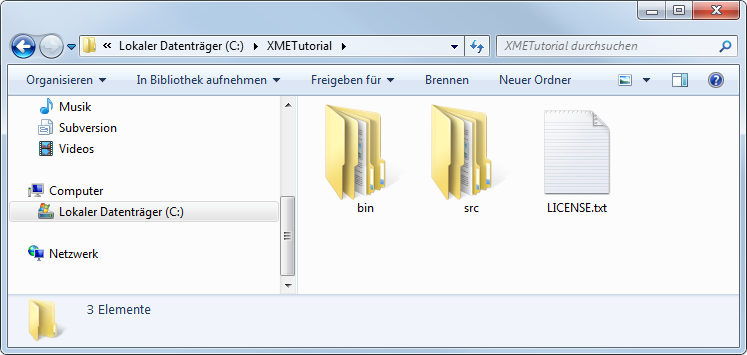
\includegraphics[scale=0.75]{figures/PNG/extracted2.png}
	\caption{Files and folders extracted from the source archive.}
	\label{fig:xme_extracted}
\end{figure}

	\item Use the \emph{start menu} to run \emph{CMake (cmake-gui)} (compare Figure~\ref{fig:cmake_run}).
	\item In the \emph{Where is the source code} field, select the full path to the directory
		\verb|<XME_ROOT>/| \verb|examples/tutorial| (compare Figure~\ref{fig:cmake_configuration1}).

\begin{figure}[htpb]
	\centering
	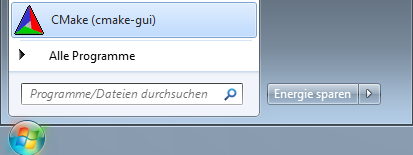
\includegraphics[scale=0.75]{figures/PNG/cmake_run.png}
	\caption{\emph{CMake (cmake-gui)} icon in the start menu.}
	\label{fig:cmake_run}
\end{figure}

\begin{figure}[htpb]
	\centering
	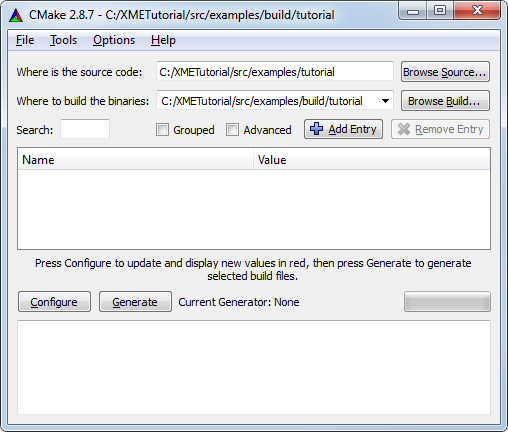
\includegraphics[scale=0.75]{figures/PNG/cmake_configuration1.png}
	\caption{Source code and build directory specification.}
	\label{fig:cmake_configuration1}
\end{figure}

	\item In the \emph{Where to build the binaries} field, select the full path to the directory
		\verb|<XME_ROOT>/| \verb|examples/build/tutorial| (note the additional \verb|build| folder,
		this folder does not yet exist).%\footnote{%
		%This will cause CMake to generate a so-called out-of-source build system, which is recommended.}
	\item Click the \emph{Configure} button.
	\item Choose the \emph{Visual Studio} toolchain that corresponds to your Visual Studio version
		(do \emph{not} use the 64 bit version) and click \emph{Finish} (compare Figure~\ref{fig:cmake_toolchain}).

\begin{figure}[htpb]
	\centering
	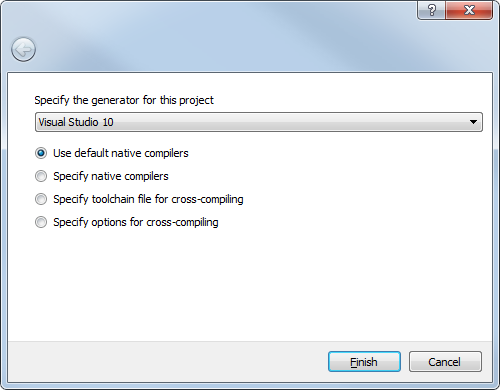
\includegraphics[scale=0.75]{figures/PNG/cmake_toolchain.png}
	\caption{Toolchain selection in CMake.}
	\label{fig:cmake_toolchain}
\end{figure}

	\item After CMake has finished its configuration, various configuration variables marked in red should appear in the list
		(compare Figure~\ref{fig:cmake_configuration2}).
	\item Click the \emph{Generate} button.
		This will generate the Visual Studio solution file \verb|Tutorial.sln| which you can open in Visual Studio.
		The file will be placed in the following directory: \verb|<XME_ROOT>/examples/build/tutorial| (compare Figure~\ref{fig:build_directory}).

\begin{figure}[h!t]
	\centering
	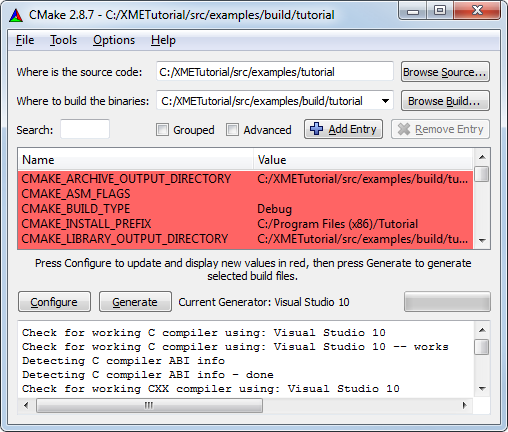
\includegraphics[scale=0.75]{figures/PNG/cmake_configuration2.png}
	\caption{Configuration and build system generation in CMake.}
	\label{fig:cmake_configuration2}
\end{figure}

\begin{figure}[htpb]
	\centering
	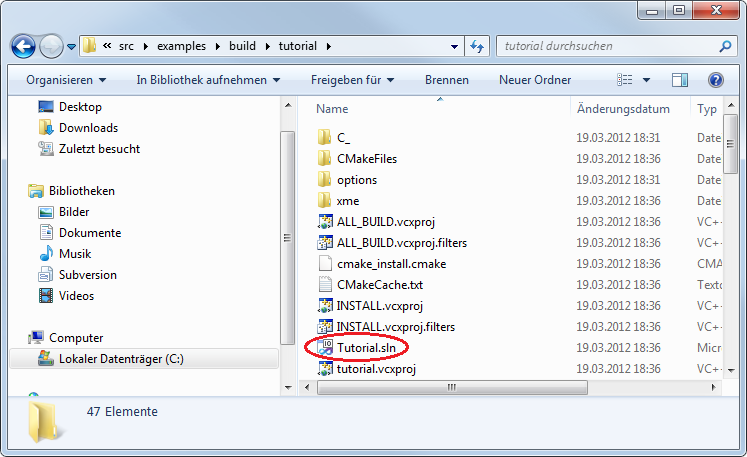
\includegraphics[scale=0.75]{figures/PNG/build_directory_edited.png}
	\caption{Build directory after build system generation, highlighted in red the Visual Studio solution file.}
	\label{fig:build_directory}
\end{figure}

\end{enumerate}

\noindent To compile the exemplified application, the following steps are required:

\begin{enumerate}
	\item Fire up Visual Studio and select \emph{File} $\rightarrow$ \emph{Open} $\rightarrow$ \emph{Project/Solution...}
	\item Navigate to the \verb|<XME_ROOT>/examples/build/tutorial| directory and select the solution file \verb|Tutorial.sln|.
	\item After loading the solution, you will see a project tree in the left-hand pane.
		Right-click on the \verb|tutorial| project and choose \emph{Set as StartUp Project}
		(compare Figure~\ref{fig:vs_set_as_startup_project}).

\begin{figure}[htpb]
	\centering
	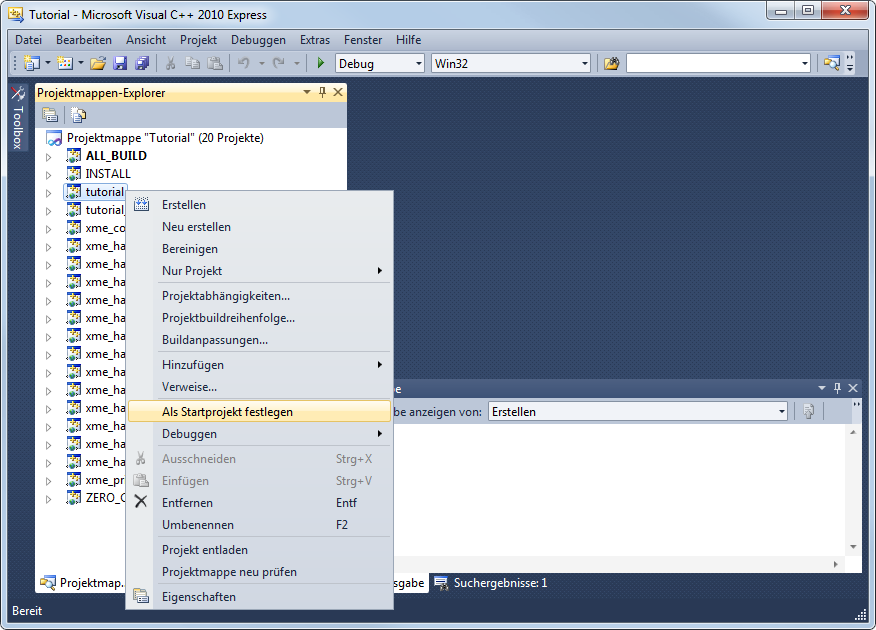
\includegraphics[scale=0.5]{figures/PNG/vs_set_as_startup_project.png}
	\caption{Setting the \texttt{tutorial} project as \emph{StartUp Project}.}
	\label{fig:vs_set_as_startup_project}
\end{figure}

	\item In the tool bar, select the solution configuration you want to build (usually \texttt{Debug} or \texttt{Release}).
		The \texttt{Debug} build includes debugging information and should be used for development.
		If in doubt, choose \texttt{Release}.

	\item Hit \emph{F7} to compile the solution.

	\item Debug/run the project as usual (e.g., hit \emph{F5} to debug or \emph{Ctrl+F5} to run without debugging).
		If you get prompted whether to rebuild the out-of-date \texttt{ZERO\_CHECK} project (compare Figure~\ref{fig:vs_zero_check}),
		you may select the \emph{Do not show this dialog box again} check box and choose \emph{Yes}.

	\item When the application starts, you will probably receive a query from the \emph{Windows Firewall}.
		\xme is designed to talk to other nodes in the network and hence needs a firewall exception for full functionality.
		If you do not want the \xme to talk to other nodes, then simply deny access.\footnote{%
		If you want to allow access to the network at a later point in time,
		you can change the Firewall settings in the \emph{System Control Panel}.}
		In this case, communication will be limited to \xme applications on the local computer.
		If you want \xme applications to communicate with each other in the local network,
		allow access to the \emph{Home or Company Network} as shown in Figure~\ref{fig:firewall_tutorial}.

\begin{figure}[htpb]
	\centering
	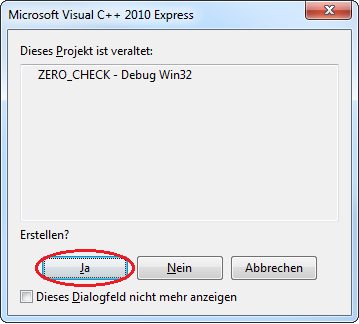
\includegraphics[scale=0.75]{figures/PNG/vs_zero_check_edited.png}
	\caption{\texttt{ZERO\_CHECK} project out of date prompt.}
	\label{fig:vs_zero_check}
\end{figure}

\begin{figure}[htpb]
	\centering
	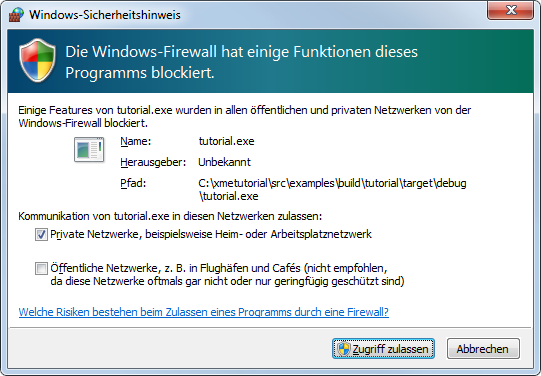
\includegraphics[scale=0.75]{figures/PNG/firewall_tutorial.png}
	\caption{Firewall settings for the \texttt{Tutorial} application.}
	\label{fig:firewall_tutorial}
\end{figure}

\end{enumerate}

This tutorial is bundled with a simple \emph{Hello World} example application, which gets built when this workflow is executed.
The entry point into the executable is in \verb|tutorial.c|, which also defines the \xme components used in this application.
The application is composed of some software components that are explained in section \ref{sec:core_components}
(\emph{Node Manager}, \emph{IP Login Server Proxy}) and an application-specific components called \emph{Hello World Component}).
The latter one prints the text ``\texttt{Hello World!}'' to the console every two seconds (compare Figure~\ref{fig:example_hello_world}).
%
You may now inspect the source code in the files \verb|tutorial.c|, \verb|helloWorldComponent.c| and \verb|helloWorldComponent.h|
to see how the concepts from Section~\ref{sec:architecture} are used in the application.

\begin{figure}[htpb]
	\centering
	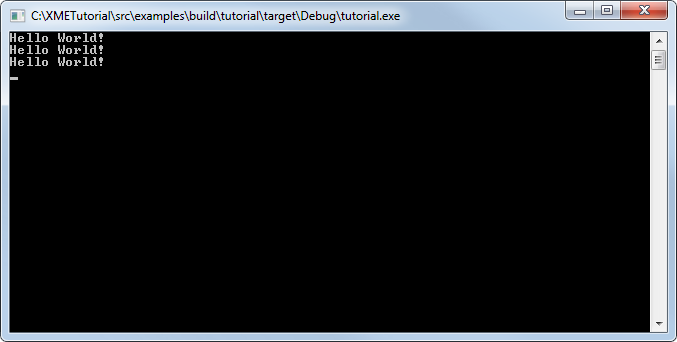
\includegraphics[scale=0.75]{figures/PNG/example_hello_world.png}
	\caption{\emph{Hello World Component} printing messages to the console.}
	\label{fig:example_hello_world}
\end{figure}

\clearpage
%
% Copyright (c) 2011-2012, fortiss GmbH.
% Licensed under the Apache License, Version 2.0.
% 
% Use, modification and distribution are subject to the terms specified
% in the accompanying license file LICENSE.txt located at the root directory
% of this software distribution. A copy is available at
% http://chromosome.fortiss.org/.
%
% This file is part of CHROMOSOME.
%
% $Id$
%
% Author:
%         Dominik Sojer <sojer@fortiss.org>
%         Michael Geisinger <geisinger@fortiss.org>
%

\section{Example 2: Chat with Chat Rooms (30 minutes)}
\label{sec:example_chat}

It is now time to replace the \emph{Hello World} application with a distributed \emph{Chat} application.
This tutorial comes with components that realize a distributed chat service.
The source code of this application is already present in the tutorial project,
we just need to configure it properly.

\begin{enumerate}
	\item The \emph{Hello World} application was using a specific component to print its ``\texttt{Hello World!}'' message.
		As this message is quite annoying in a chat room, we first have to remove the \emph{Hello World} component from the tutorial project.
		At the same time, we enable the \emph{Chat Component} which implements the chat client.
		This has to be done in the project's main file {\tt tutorial.c},
		which can be opened in Visual Studio by double-clicking on the respective item
		below \emph{tutorial} $\rightarrow$ \emph{Source Files} in the \emph{Project Explorer} pane.
		Please comment the line with the {\tt helloWorldComponent}
		and uncommend (enable) the line with the {\tt chatComponent} as shown below:

\begin{lstlisting}[numbers=left,firstnumber=48]
/*************************************************************************/
/***   Component descriptor                                            ***/
/*************************************************************************/
XME_COMPONENT_LIST_BEGIN
	XME_COMPONENT_LIST_ITEM(xme_core_nodeManager, 0)
	XME_COMPONENT_LIST_ITEM(xme_prim_ipLoginServerProxy, 0)
/*	XME_COMPONENT_LIST_ITEM(helloWorldComponent, 0)*/ /~~/ Comment this line
	XME_COMPONENT_LIST_ITEM(chatComponent, 0)       /~~/ Uncomment this line
XME_COMPONENT_LIST_END;
\end{lstlisting}

	\item The routing of messages is performed automatically by \xme core components.
		To keep the tutorial project small, all required components for network management and routing messages
		between distributed nodes (i.e., \emph{Login Server} and \emph{Master Directory}) have been added to a separate project named {\bf Coordinator}.
		We will treat the Coordinator as a separate node and have it running in the background so that people can dynamically enter chat rooms.
		
		To be able to use this functionality, please go go back to Section~\ref{sec:example_helloworld}
		and perform the described steps again for the \verb|coordinator| example.
		Please use the directory \verb|<XME_ROOT>/| \verb|examples/coordinator| as input for the \emph{Where is the source code} field
		and use the directory \verb|<XME_ROOT>/examples/build/coordinator| as input for the
		\emph{Where to build the binaries} field within CMake.
		After generation of the build system, the \verb|Coordinator.sln| Visual Studio solution file
		can be found in at \verb|<XME_ROOT>/examples/build/coordinator|.
		Do not forget to set up \verb|coordinator| as the \emph{StartUp Project} within Visual Studio.
		
	\item After having successfully compiled the coordinator project as well as the tutorial project,
		a basic distributed chat application can be started.
		In order to do this, execute {\bf one instance} of the coordinator application.
		If you receive a request from the \emph{Windows Firewall},
		please allow communication to the \emph{Home or Company Network} as shown in Figure~\ref{fig:firewall_coordinator}.
		Note that if you have colleagues on the same network running this tutorial at the same time,
		you should talk to them to only run one instance of the Coordinator at any point in time.\footnote{%
			This is a limitation of the current version of \xme. We do not yet support multiple subnets
			or detect the presence of other Coordinator instances. This will change in future versions.}
		
		The Coordinator can either be started from Visual Studio or by executing \verb|<XME_ROOT>/|
		\verb|examples/build/coordinator/target/*/coordinator.exe|.
		This will open a terminal window in which \xme may print logging information.
		By default, the log level is set up so that only warnings and errors will be shown,
		so it is normal for the terminal window to not show any activity.

\begin{figure}[htpb]
	\centering
	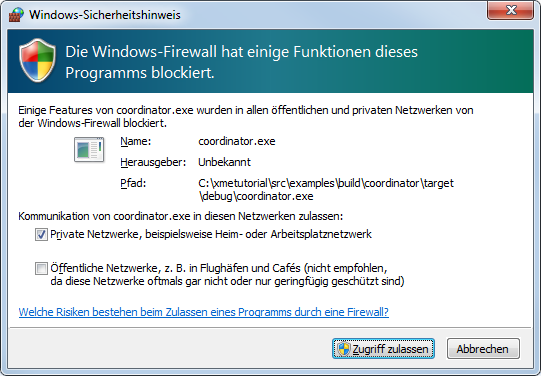
\includegraphics[scale=0.75]{figures/PNG/firewall_coordinator.png}
	\caption{Firewall settings for the \texttt{Coordinator} application.}
	\label{fig:firewall_coordinator}
\end{figure}

	\item We can now execute an arbitrary number of instances of the tutorial application.
		To do this, navigate to the respective directory and launch
		\verb|<XME_ROOT>/examples/build/| \verb|tutorial/target/*/tutorial.exe|.
		This will also open a terminal window, which first prompts to enter a name.
		After a name is given, you will be presented a list of commands and chat rooms to choose from
		(compare Figure~\ref{fig:example_chat}).

\begin{figure}[htpb]
	\centering
	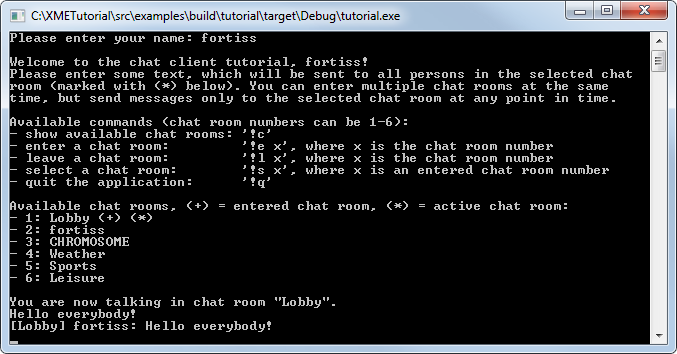
\includegraphics[scale=0.75]{figures/PNG/example_chat.png}
	\caption{Sending chat messages via the \emph{Chat Component}.}
	\label{fig:example_chat}
\end{figure}

		The semantics of a chat room are that messages sent to a chat room should only be visible to people that have joined the respective chat room.
		This concept can be directly mapped to the notion of \emph{topics}.
		
		Anything that is not a command is interpreted as a message to send to the \emph{active} chat room.
		The active chat room can be changed with the \texttt{!s} command.
		
		Launch multiple instances of the chat example using different names and send some messages.
		Then run the application in a distributed way using multiple computers on the same subnet.

\end{enumerate}

\clearpage
%
% Copyright (c) 2011-2012, fortiss GmbH.
% Licensed under the Apache License, Version 2.0.
% 
% Use, modification and distribution are subject to the terms specified
% in the accompanying license file LICENSE.txt located at the root directory
% of this software distribution. A copy is available at
% http://chromosome.fortiss.org/.
%
% This file is part of CHROMOSOME.
%
% $Id$
%
% Author:
%         Dominik Sojer <sojer@fortiss.org>
%         Michael Geisinger <geisinger@fortiss.org>
%

\section{Example 3: Chat Calculator (20+ minutes)}
\label{sec:example_chatcalculator}

After having modified an already existing component in Section~\ref{sec:example_chat},
it is now time to create a completely new component.
%
A so-called \emph{Chat Calculator} component is a good starting point for digging deeper into \xme.
%
The calculator should fulfill the following requirements:
\begin{itemize}
	\item Join a chat room.
	\item Announce its presence in the chat room every 30 seconds.
	\item Listen to commands of the form ``\verb|!calc <operand1> <operation> <operand2>|''.
	\item Support addition, subtraction, multiplication and divison as \verb|<operation>|.
	\item Send calculated results to the chat room in the form\\
		``\verb|<operand1> <operation> <operand2> = <result>|''.
	\item Gracefully handle division by zero.
\end{itemize}

The following steps guide you through the implementation of the \emph{Calculator Component}.
Please be warned that the given time frame of 20 minutes does not include thorough reading and understanding of the code.
You can find electronic versions of the code for the \emph{Calculator Component} on the \xme website\footnote{%
\url{http://chromosome.fortiss.org/}}.

\begin{enumerate}
	\item Use the \emph{Template Generator} application to create a new component with name ``\texttt{Chat Calculator}'' of class \verb|adv| (advanced).
		The \emph{Template Generator} application can be found in the directory \verb|<XME_ROOT>/../bin/windows_x86| and is explained in FAQ~\ref{faq:create_component}.
		
		The application will generate two files named \verb|chatCalculator.h| and \verb|chatCalculator.c|
		in the directory \verb|<XME_ROOT>/xme/adv| and fill it with sample content.
		Furthermore, it will automatically add the new component to the \verb|CMakeLists.txt| file in the same directory.
		This is the quickest way to generate a new \xme component.

%	\item First, we need to decide whether the new component will be a member of the class \texttt{adv} (advanced),
%		\texttt{prim} (primitive) or \texttt{hal} (hardware abstraction).
%		These classes define how the component can communicate with other components.
%		Application components like the \emph{Calculator Component} are typically \emph{advanced},
%		which means that they can exchange data with other application components only using data centric communication.
%		We choose \verb|xme_adv_chatCalculator| as our component name.
%
%	\item Create a C source and header file in the coresponding folder \verb|<XME_ROOT>/| \verb|xme/adv|,
%		and name it \verb|xme_|\textsf{\itshape class}\verb|_|\textsf{\itshape name}, where \textsf{\itshape name} is the name of the component,
%		preferably in \texttt{camelCaseWriting} style if the name consists of multiple words.

%	\item In the folder where the new header and source file is located,
%		edit \verb|CMakeLists.txt| and insert the new component into the list:
%
%\begin{lstlisting}[numbers=left,firstnumber=18]
%xme_add_component(   # Add this block
%	"xme_adv_chatCalculator"
%	chatCalculator.h chatCalculator.c
%)
%\end{lstlisting}

	\item Edit the \verb|CMakeLists.txt| file of the \verb|<XME_ROOT>/examples/tutorial| project to use the new component:

\begin{lstlisting}[language=cmake,numbers=left,firstnumber=62]
# Build XME components
xme_link_components(
	"tutorial"
	xme_prim_ipLoginServerProxy
	xme_core_core
	xme_hal_dio
	xme_hal_net
	xme_hal_sleep
	xme_adv_chatCalculator   ~\char"0023~ Add this line
)
\end{lstlisting}

		Note that CMake will automatically pick up the changes in \verb|CMakeLists.txt| when we perform the next full compile.
		This is why you do not have to rerun CMake manually after this change.

	\item Open the \verb|Tutorial| solution with the modifications from Section~\ref{sec:example_chat} in \emph{Visual Studio}
		and edit \verb|tutorial.c| to include the new component:

	\begin{lstlisting}[numbers=left,firstnumber=25]
/*************************************************************************/
/***   Includes                                                        ***/
/*************************************************************************/
#include "chatComponent.h"
#include "helloWorldComponent.h"
#include "xme/core/componentList.h"
#include "xme/prim/ipLoginServerProxy.h"
#include "xme/adv/chatCalculator.h"   /~~/ Add this line
\end{lstlisting}

	\item Declare the component configuration and add an instance of the component
		to the component list in \verb|tutorial.c|. Apply the following two modifications:

\begin{lstlisting}[numbers=left,firstnumber=48]
/*************************************************************************/
/***   Component configurations                                        ***/
/*************************************************************************/
XME_COMPONENT_CONFIG_INSTANCE(xme_core_nodeManager) =
{
	0x00000000021041A1, // deviceType
	XME_CORE_DEVICE_GUID_RANDOM // deviceGuid
};

XME_COMPONENT_CONFIG_INSTANCE(xme_prim_ipLoginServerProxy, 1);

XME_COMPONENT_CONFIG_INSTANCE(helloWorldComponent, 1);

XME_COMPONENT_CONFIG_INSTANCE(chatComponent, 1);

XME_COMPONENT_CONFIG_INSTANCE(xme_adv_chatCalculator) = /~~/ Add this block
{
	// public
	CHAT_TOPIC_BASE // topic
};

/*************************************************************************/
/***   Component descriptor                                            ***/
/*************************************************************************/
XME_COMPONENT_LIST_BEGIN
	XME_COMPONENT_LIST_ITEM(xme_core_nodeManager, 0)
	XME_COMPONENT_LIST_ITEM(xme_prim_ipLoginServerProxy, 0)
//	XME_COMPONENT_LIST_ITEM(helloWorldComponent, 0)
	XME_COMPONENT_LIST_ITEM(chatComponent, 0)
	XME_COMPONENT_LIST_ITEM(xme_adv_chatCalculator, 0)   /~~/ Add this line
XME_COMPONENT_LIST_END;
\end{lstlisting}

	\item After these changes, press \emph{F7} in \emph{Visual Studio} to build the solution.
		This is required for CMake to pick up the changes in the build system.
		You will probably notice CMake re-run automatically in the \emph{Visual Studio} console.
		You might be prompted whether to reload the \emph{Visual Studio Solution}, in which case you should choose \emph{Reload}
		(compare Figure~\ref{fig:vs_detect_change_tutorial}).

\begin{figure}[htpb]
	\centering
	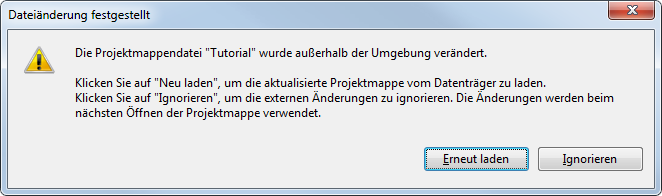
\includegraphics[scale=0.75]{figures/PNG/vs_detect_change_tutorial.png}
	\caption{\emph{Visual Studio Solution} reload prompt after \emph{CMake} has regenerated the build system.}
	\label{fig:vs_detect_change_tutorial}
\end{figure}

	\item You should now see the \verb|xme_adv_chatCalculator| item in the \emph{Project Navigator} pane in \emph{Visual Studio}.
		You can comfortably edit the source and header file of the component from there.

\begin{figure}[htpb]
	\centering
	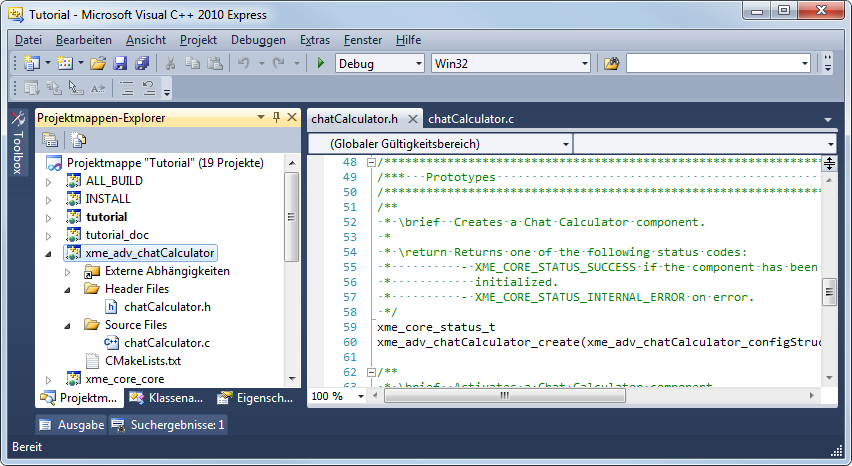
\includegraphics[width=\textwidth]{figures/PNG/vs_chatCalculator.png}
	\caption{\texttt{xme\_adv\_chatCalculator} component in the \emph{Visual Studio Project Navigator} pane.}
	\label{fig:vs_chatCalculator}
\end{figure}

	\item The component we have just added comes with some example code that we have to adapt in order to implement the \emph{Chat Calculator}.
		Open the respective files \verb|chatCalculator.h| and \verb|chatCalculator.c| found in \verb|<XME_ROOT>/xme/adv| to make yourself familiar with the generated code.
		You will notice that the generated example code publishes and subscribes the \verb|XME_CORE_TOPIC_EVENT| topic
		and that a task is created that prints a message every two seconds.
		The publication and subscription handles as well as the task handle is stored in the component's configuration structure \verb|xme_adv_chatCalculator_configStruct_t|.
		
		We can reuse the existing functionality for implementing the \emph{Chat Calculator},
		because the calculator has to listen (read: subscribe) to a specific chat room
		and print (read: publish) the result of the calculation.
		Furthermore, we need to announce the presence of the \emph{Chat Calculator} every 30~seconds,
		for which the task can be used.
		
		In order to ensure maximum flexibility (and to demonstrate how to use configuration variables),
		we will configure the topic of the chat room to enter (i.e., the topic) in \emph{Chat Calculator}'s configuration.
		For this, we will define a member variable called \verb|topic| in the comfiguration structure
		that we can set to an arbitrary value in our main program when we instantiate the component.
		In \verb|chatCalculator.h|, apply the following two changes:

\begin{lstlisting}[numbers=left,firstnumber=33]
/*************************************************************************/
/***   Type definitions                                                ***/
/*************************************************************************/
typedef struct
{
	// public
	xme_core_topic_t topic;                             /~~/ Change this line
	// private
/*	int dummyState; */                       /~~/ Comment or remove this line
	xme_core_resourceManager_taskHandle_t taskHandle;
	xme_core_dcc_publicationHandle_t publicationHandle;
	xme_core_dcc_subscriptionHandle_t subscriptionHandle;
}
xme_adv_chatCalculator_configStruct_t;
\end{lstlisting}

		We can leave the rest of the header file as-is.

	\item Now it is time to implement the actual functionality in \verb|chatCalculator.c|.
		Start by changing the published and subscribed topic to the chat room in which we want the \emph{Chat Calculator} to be.
		Apply the following four changes:

\begin{lstlisting}[numbers=left,firstnumber=69]
xme_core_status_t
xme_adv_chatCalculator_create(xme_adv_chatCalculator_configStruct_t* config)
{
	// TODO: Initialize component state
/*	config->dummyState = 0; */               /~~/ Comment or remove this line

/*	// TODO: Add code */                    /~~/ Comment or remove this block
//	XME_LOG(XME_LOG_NOTE, "Create function of Chat Calculator called!\n");

	// Example: Publish a topic
	config->publicationHandle =
		xme_core_dcc_publishTopic
		(
			config->topic,                              /~~/ Change this line
			XME_CORE_MD_EMPTY_META_DATA,
			false,
			NULL
		);

	// Check for errors
	if (XME_CORE_DCC_INVALID_PUBLICATION_HANDLE == ~\LstSuppressNumber~
		                                         config->publicationHandle) ~\LstReactivateNumber~
	{
		return XME_CORE_STATUS_INTERNAL_ERROR;
	}

	// Example: Subscribe to a topic
	config->subscriptionHandle =
		xme_core_dcc_subscribeTopic
		(
			config->topic,                              /~~/ Change this line
			XME_CORE_MD_EMPTY_META_DATA,
			false,
			_xme_adv_chatCalculator_receiveDataCallback,
			config
		); ~\LstSuppressNumber~

	[...]                           /~~/ Leave the rest of the function as-is
} ~\LstReactivateNumber~
\end{lstlisting}

	\item Now we should adapt the \verb|_xme_adv_chatCalculator_receiveDataCallback()| function,
		which handles incoming data for the subscribed topic:

\begin{lstlisting}[numbers=left,firstnumber=28]
/*************************************************************************/
/***   Implementation                                                  ***/
/*************************************************************************/
// TODO: Use or remove this sample topic subscription callback function:
static
void
_xme_adv_chatCalculator_receiveDataCallback(xme_hal_sharedPtr_t dataHandle, ~\LstSuppressNumber~
                                                            void* userData) ~\LstReactivateNumber~
{
	// TODO: In case you supply the component's configuration instance
	//       via userData when subscribing, you can access it here:
	xme_adv_chatCalculator_configStruct_t* config = ~\LstSuppressNumber~
                          (xme_adv_chatCalculator_configStruct_t*)userData; ~\LstReactivateNumber~

/*	// TODO: Add code */                    /~~/ Comment or remove this block
//	XME_LOG(XME_LOG_NOTE, "Receive data callback function called!\n");
	
/*	// Example: Print data to screen */     /~~/ Comment or remove this block
//	{
//		const char* message = xme_hal_sharedPtr_getPointer(dataHandle);
//		XME_LOG(XME_LOG_NOTE, "Received: %s\n", message);
//	}

	/~~/ Add all the following lines

	char* input = (char*)xme_hal_sharedPtr_getPointer(dataHandle);
	int size = xme_hal_sharedPtr_getSize(dataHandle);

	// Output data
	char output[512];

	// Sanitize input
	input[size-1] = 0;

	// Strip person's name
	input = strchr(input, ':');
	if (NULL == input)
	{
		// Invalid message format
		return;
	}
	input += 2;

	if (0 != strncmp(input, "!calc ", 6))
	{
		// Not a calculation command
		return;
	}

	_xme_adv_chatCalculator_getResultString
	(
		input, output, sizeof(output)
	);

	if (0 != strlen(output))
	{
		xme_core_dcc_sendTopicData
		(
			config->publicationHandle,
			(void*)output, strlen(output)+1
		);
	}
}
\end{lstlisting}

	\item Add the \verb|_xme_adv_chatCalculator_getResultString()| function, which calculates the result of an operation,
		above \verb|_xme_adv_chatCalculator_receiveDataCallback()|:

\begin{lstlisting}[numbers=left,firstnumber=31]
static
void
_xme_adv_chatCalculator_getResultString(char* in, char* out, int outSize)
{
	// Error messages
	const char* error_syntax = "The expression could not be evaluated";
	const char* error_zero = "Division by zero";
	const char* error_op = "Invalid operator";

	double operand1, operand2, result;
	char op;
	char* pos;

	// Parse string
	pos = strchr(in, 0x20);
	if (NULL == pos)
	{
		strcpy_s(out, outSize, error_syntax);
		return;
	}
	operand1 = atof(pos+1);

	pos = strchr(pos+1, 0x20);
	if (NULL == pos)
	{
		strcpy_s(out, outSize, error_syntax);
		return;
	}
	op = *(pos+1);
	
	// Ignore own announcement message
	if ('<' == op)
	{
		out[0] = 0;
		return;
	}

	pos = strchr(pos+1, 0x20);
	if (NULL == pos)
	{
		strcpy_s(out, outSize, error_syntax);
		return;
	}
	operand2 = atof(pos+1);

	// Check for operator and division by zero
	if (!_xme_adv_chatCalculator_isOperationValid(op))
	{
		strcpy_s(out, outSize, error_op);
		return;
	}
	if (_xme_adv_chatCalculator_isDivisionByZero(op, operand2))
	{
		strcpy_s(out, outSize, error_zero);
		return;
	}

	// Calculate result
	result =
		_xme_adv_chatCalculator_calculateResult(operand1, op, operand2);

	// Output result
	sprintf_s
	(
		out, outSize, "%lf %c %lf = %lf",
		operand1, op, operand2, result
	);
}
\end{lstlisting}

	\item Add the following two includes to \verb|chatCalculator.c|:
	
\begin{lstlisting}[numbers=left,firstnumber=23]
/*************************************************************************/
/***   Includes                                                        ***/
/*************************************************************************/
#include "xme/adv/chatCalculator.h"

#include <~\texttt{float}~.h>                                          /~~/ Add this line
#include <math.h>                                          /~~/ Add this line
\end{lstlisting}

	\item Add the following helper functions above \verb|_xme_adv_chatCalculator_getResultString()|:

\begin{lstlisting}[numbers=left,firstnumber=34]
static
bool
_xme_adv_chatCalculator_isOperationValid(char operation)
{
	return ('+' == operation || '-' == operation ||
		'/' == operation || '*' == operation);
}

static
bool
_xme_adv_chatCalculator_isDivisionByZero(char operation, double operand2)
{
	return ('/' == operation && abs(operand2) < DBL_EPSILON);
}

static
double
_xme_adv_chatCalculator_calculateResult(double operand1, char operation,
                                                         double operand2)
{
	if ('+' == operation)
	{
		return operand1 + operand2;
	}
	if ('-' == operation)
	{
		return operand1 - operand2;
	}
	if ('*' == operation)
	{
		return operand1 * operand2;
	}
	if ('/' == operation)
	{
		// Division by zero is handled in isDivisionByZero()
		return operand1 / operand2;
	}

	// Invalid operation is handled in isOperationValid()
	return 0;
}
\end{lstlisting}

	\item Change the text the task sends to the chat room and remove debug output:

\begin{lstlisting}[numbers=left,firstnumber=205]
// TODO: Use or remove this sample task callback function:
static
void
_xme_adv_chatCalculator_taskCallback(void* userData)
{
	// TODO: In case you supply the component's configuration instance
	//       via userData when creating the task, you can access it here:
	xme_adv_chatCalculator_configStruct_t* config = ~\LstSuppressNumber~
                          (xme_adv_chatCalculator_configStruct_t*)userData; ~\LstReactivateNumber~

/*	// TODO: Add code */                    /~~/ Comment or remove this block
//	XME_LOG(XME_LOG_NOTE, "Task callback function called!\n");

	// Example: Send data
	{                                         /~~/ Change the following lines
		static const char* message = "Chat Calculator awaiting commands.\n"
			"Usage: !calc <operand1> <operation> <operand2>"; ~\LstSuppressNumber~
		[...]                       /~~/ Leave the rest of the function as-is
	}
} ~\LstReactivateNumber~
\end{lstlisting}

	\item Configure the task to fire every 30 seconds instead of every two seconds
		and remove debug output:

\begin{lstlisting}[numbers=left,firstnumber=272]
xme_core_status_t
xme_adv_chatCalculator_activate(xme_adv_chatCalculator_configStruct_t* config)
{
/*	// TODO: Add code */                    /~~/ Comment or remove this block
//	XME_LOG(XME_LOG_NOTE, "Activate function of Chat Calculator called!\n");

	// Example: Start a task:
	config->taskHandle =
		xme_core_resourceManager_scheduleTask
		(
			1000,
			30000,                                      /~~/ Change this line
			XME_HAL_SCHED_PRIORITY_NORMAL,
			_xme_adv_chatCalculator_taskCallback,
			config
		); ~\LstSuppressNumber~

	[...]                           /~~/ Leave the rest of the function as-is
} ~\LstReactivateNumber~
\end{lstlisting}

	\item Finally, remove some more debug output:

\begin{lstlisting}[numbers=left,firstnumber=298]
void
xme_adv_chatCalculator_deactivate(xme_adv_chatCalculator_configStruct_t* config)
{
/*	// TODO: Add code */                    /~~/ Comment or remove this block
//	XME_LOG(XME_LOG_NOTE, "Deactivate function of Chat Calculator called!\n"); ~\LstSuppressNumber~

	[...]                       /~~/ Leave the rest of the function as-is
} ~\LstReactivateNumber~
\end{lstlisting}

\begin{lstlisting}[numbers=left,firstnumber=308]
void
xme_adv_chatCalculator_destroy(xme_adv_chatCalculator_configStruct_t* config)
{
/*	// TODO: Add code */                    /~~/ Comment or remove this block
//	XME_LOG(XME_LOG_NOTE, "Destroy function of Chat Calculator called!\n"); ~\LstSuppressNumber~

	[...]                       /~~/ Leave the rest of the function as-is
} ~\LstReactivateNumber~
\end{lstlisting}

	\item That's it! Compile and run the \verb|tutorial| example (press \emph{F7} and \emph{F5} in \emph{Visual Studio}).
		Test the new component by letting the \emph{Chat Calculator} do your math homework ;)
\end{enumerate}

\section{More Examples}

You might consider implementing the following components to get to know \xme even better:
\begin{itemize}
	\item A ``spammer'' component that sends unsolicited advertisements to chat channels.
	\item A component that keeps track of all persons in each chat room and supports a ``\verb|!who|'' command to print a list
		(you might want to extend the \emph{Chat Example} to publish additional data in order to do this).
	\item A ``lunch time'' component that announces lunch time at noon in every chat room.
\end{itemize}

%\section{Questions to Reviewers}
%\begin{enumerate}
%	\item Are the given timeframes for finishing every section realistic?
%	\item Does Sec. \ref{sec:intro} (``Introduction'') provide you any valuable information? What else did you expect something else there?
%	\item Did you encounter any inconsistencies between this tutorial and the actual source code?
%	\item Did you get enough / the right information from Sec. \ref{sec:architecture} (``XME in a Nutshell'')?
%	\item Is the gap between Sec. \ref{sec:chatExample} (``Chat Example'') and Sec. \ref{sec:xchat} (``Extended Chat Example'') too big?
%	\item Did you encounter any other \emph{noticeable} situations, while working through this tutorial?
%\end{enumerate}

\clearpage
\appendix

%
% Copyright (c) 2011-2012, fortiss GmbH.
% Licensed under the Apache License, Version 2.0.
% 
% Use, modification and distribution are subject to the terms specified
% in the accompanying license file LICENSE.txt located at the root directory
% of this software distribution. A copy is available at
% http://chromosome.fortiss.org/.
%
% This file is part of CHROMOSOME.
%
% $Id$
%
% Author:
%         Michael Geisinger <geisinger@fortiss.org>
%

\section{Frequently Asked Questions}
\label{appx:faq}

\subsection{Technical Questions}

\subsubsection{How can I create a new component?}
\label{faq:create_component}

\xme comes with an application that can create template files for new components.
This application is called \verb|templateGenerator| and can be found in the \verb|bin/windows_x86|
subdirectory of the release package or built manually just like any other \xme example program (see Section~\ref{sec:example_helloworld} for hints).

The application will ask you for the component name, type as well as your name (for the author field)
and generate a header and a source file for the new component in the respective directory (compare Figure~\ref{fig:example_templateGenerator}).
Consider using one of the existing example applications for testing your new component if application, see Section~\ref{sec:example_chatcalculator}
for more information on how to embed a new component into an existing application.

\begin{figure}[htbp]
	\centering
	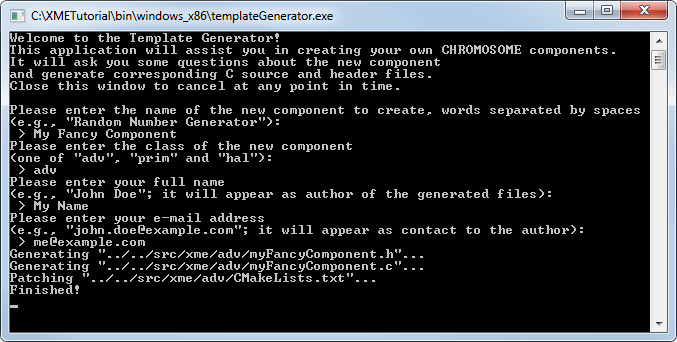
\includegraphics[scale=0.75]{figures/PNG/example_templateGenerator.png}
	\caption{\emph{Template Generator} in action.}
	\label{fig:example_templateGenerator}
\end{figure}

\subsubsection{How can I define a new topic?}

Topic identifiers are simple numbers with associated semantics.
The \verb|xme_core_topic_t| type defined in file \verb|<XME_ROOT>/xme/core/topic.h| declares some generic topic identifiers.
Topic numbers in the range between zero and \verb|XME_CORE_TOPIC_USER|-1 are reserved for internal use.
This means that you can define a new topic by using an arbitrary number larger or equal to \verb|XME_CORE_TOPIC_USER|.

Note that there is currently no mechanism in place for checking that the same topic identifiers are always used for the same type of data.
Be aware that other people in the same network might use the same topic identifiers for their data.
We plan to put a mechanism in place for avoiding this issue in future versions of \xme.

\subsubsection{How can I port \xme to my own target platform?}

The current release of \xme supports only Windows.
However, we are in the process of developing platform support layers for other platforms.
These include Linux, medium-sized microcontroller platforms like ARM Cortex M3 (e.g., as central control units)
as well as low-end microcontrollers like Atmel AVR (e.g., for sensor networks).
Upcoming releases of \xme will ship with the respective functionality.

If you favorite platform is not on this list, there are multiple options:
\begin{enumerate}
	\item You can suggest \xme to be ported onto your platform.
		If your application is of high relevance, we might indeed port \xme to that platform.
	
	\item You can contribute to the development of \xme and have your platform supported as a target platform.
	
	\item You can take the \xme source code and implement the respective platform support without revealing the source code.
		Our license model permits this (see also Appendix~\ref{appx:license}).
\end{enumerate}

\subsection{Conceptual Questions}

\subsubsection{How do you want to implement semantic aspects?}

Current middleware technology lacks semantic integration.
We are using a data-centric design, where we describe the data with an ontology.
If several domains are involved, there might be the necessity to map between the domain-specific ontologies.
This must be done manually, but can be reused (and must therefore be done only once).

% Thoughts (CB):
% Actually I am not sure, whether we really need a full-blown ontology.
% Most probably a list of available data classes is enough.
% In addition a good structuring (e.g. in the automotive area according to the different domains) might be useful.

\subsubsection{How do you specify extra-functional requirements?}

We use meta-data to describe concrete data sources.
Examples for meta-data are accuracy, confidence level, age.
In addition, we want to use application patterns to describe the extra-functional properties of concrete applications.

\subsubsection{How do you guarantee extra-functional requirements?}

We focus on implementations that can easily guarantee these requirements (e.g., time-triggered execution).
If we have more flexible protocols, we have two options: either we cannot guarantee requirements or we have to be more pessimistic.

% Thoughts (CB):
% Our main advantage is that we know the requirements (even at run-time).
% In todays systems, the only thing that the system knows at run-time is the configuration that was derived by the requirements.
% However, the concrete motivation for a specific solution is not available at run-time.
% Hence, the system cannot properly react if something goes wrong (good example: run-time monitoring of assumptions is typically not done).

\clearpage
%
% Copyright (c) 2011-2012, fortiss GmbH.
% Licensed under the Apache License, Version 2.0.
% 
% Use, modification and distribution are subject to the terms specified
% in the accompanying license file LICENSE.txt located at the root directory
% of this software distribution. A copy is available at
% http://chromosome.fortiss.org/.
%
% This file is part of CHROMOSOME.
%
% $Id$
%
% Author:
%         Michael Geisinger <geisinger@fortiss.org>
%

\section{Installing Visual C++ 2010 Express}
\label{appx:install_vs}

Follow these steps to install Visual C++ 2010 Express:

\begin{enumerate}
	\item Point your faviorite browser to
		\url{http://www.microsoft.com/visualstudio/en-us/products/2010-editions/visual-cpp-express}
		(compare Figure~\ref{fig:setup_vs_download1}).

\begin{figure}[htbp]
	\centering
	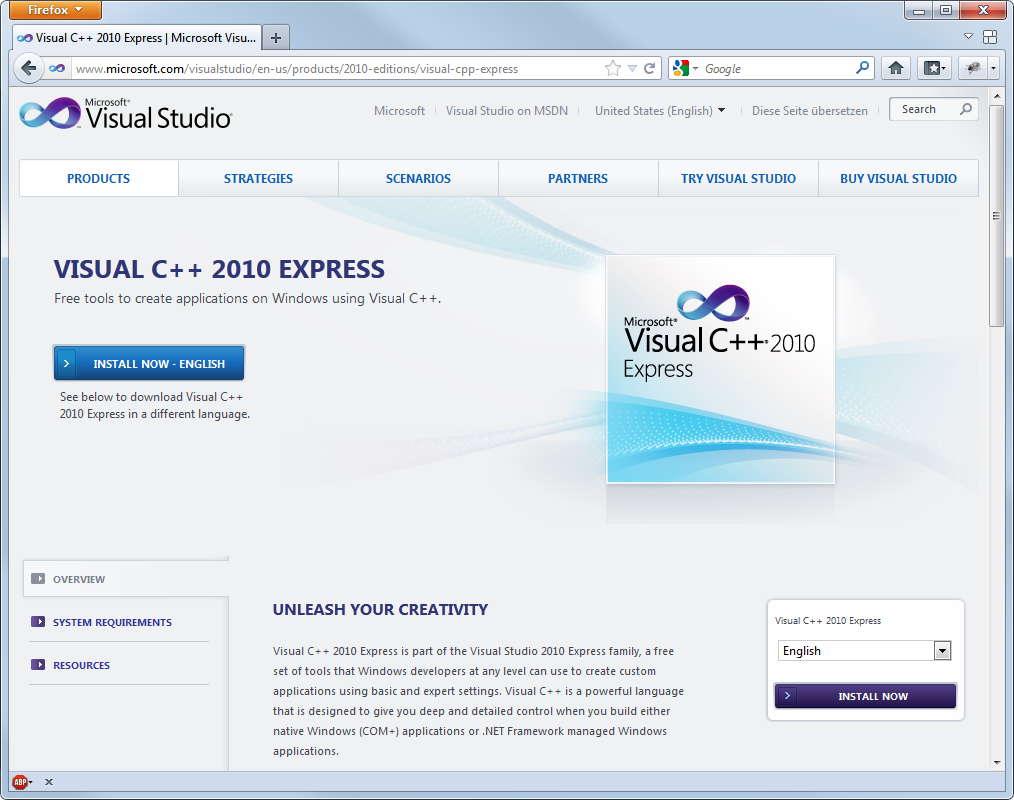
\includegraphics[scale=0.45]{figures/PNG/setup_vs_download1.png}
	\caption{Selecting Visual C++ 2010 Express for download.}
	\label{fig:setup_vs_download1}
\end{figure}

	\item Choose your language and click on \emph{Install}.
	
	\item If you are asked whether you want to install Visual Studio 2011 Professional instead,
		choose \emph{Visual C++ 2010 Express (English)} (compare Figure~\ref{fig:setup_vs_download2})\footnote{
		Alternatively, you can use the following direct link:\\
		\url{http://download.microsoft.com/download/1/D/9/1D9A6C0E-FC89-43EE-9658-B9F0E3A76983/vc_web.exe}}.

\begin{figure}[htbp]
	\centering
	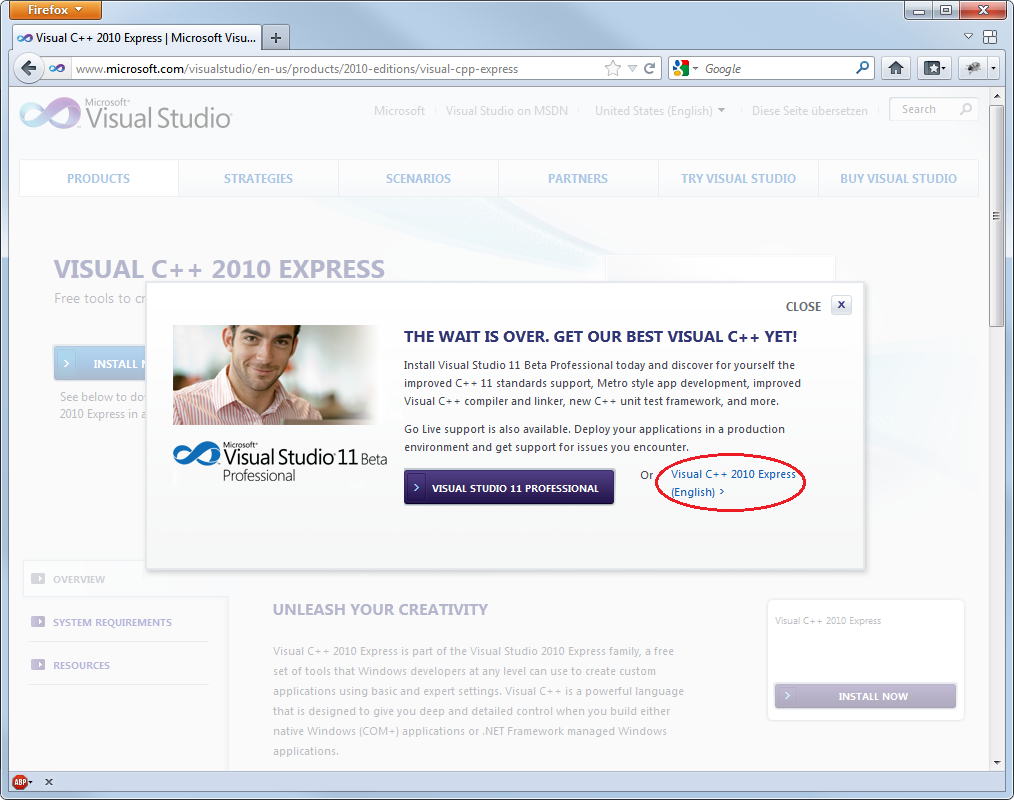
\includegraphics[scale=0.45]{figures/PNG/setup_vs_download2_edited.png}
	\caption{Downloading Visual C++ 2010 Express, highlighted in red the download link.}
	\label{fig:setup_vs_download2}
\end{figure}

	\item After downloading \texttt{vc\_web.exe}, launch it.
		Read the welcome screen and click \emph{Next} when ready. % (Figure~\ref{fig:setup_vs_welcome}).

%\begin{figure}[htbp]
%	\centering
%	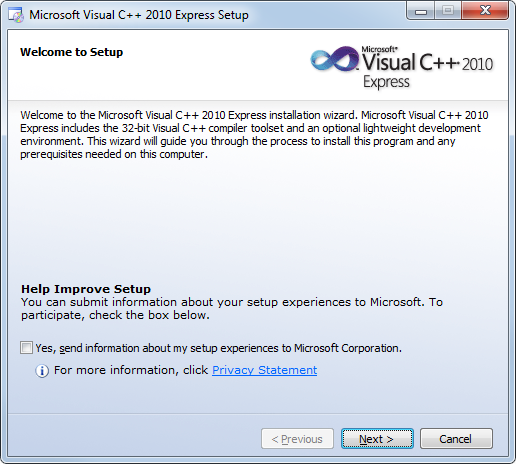
\includegraphics[scale=0.75]{figures/PNG/setup_vs_welcome.png}
%	\caption{Visual C++ 2010 Express setup welcome screen.}
%	\label{fig:setup_vs_welcome}
%\end{figure}

	\item Read the terms and conditions and choose the appropriate option. % (Figure~\ref{fig:setup_vs_terms}).

%\begin{figure}[htbp]
%	\centering
%	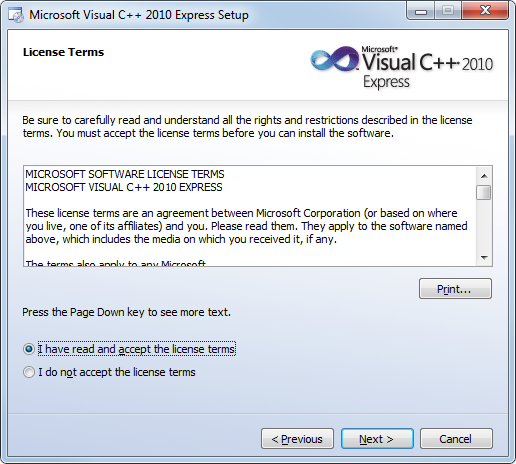
\includegraphics[scale=0.75]{figures/PNG/setup_vs_terms.png}
%	\caption{Visual C++ 2010 Express license terms.}
%	\label{fig:setup_vs_terms}
%\end{figure}

	\item On the \emph{Installation Options} page, you may deselect \emph{Silverlight} and \emph{SQL Server 2008}, they are not needed for \xme (Figure~\ref{fig:setup_vs_optional}).

\begin{figure}[htbp]
	\centering
	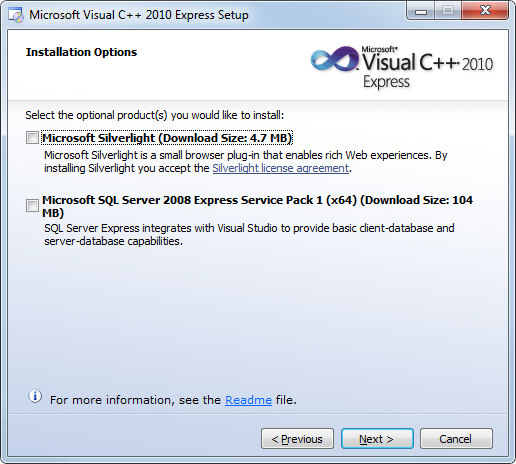
\includegraphics[scale=0.75]{figures/PNG/setup_vs_optional.png}
	\caption{Visual C++ 2010 Express installation options.}
	\label{fig:setup_vs_optional}
\end{figure}

	\item On the \emph{Destination Folder} page, select the installation directory.
		In some cases, you might not be able to choose a directory manually. % (compare Figure~\ref{fig:setup_vs_destination}).

%\begin{figure}[htbp]
%	\centering
%	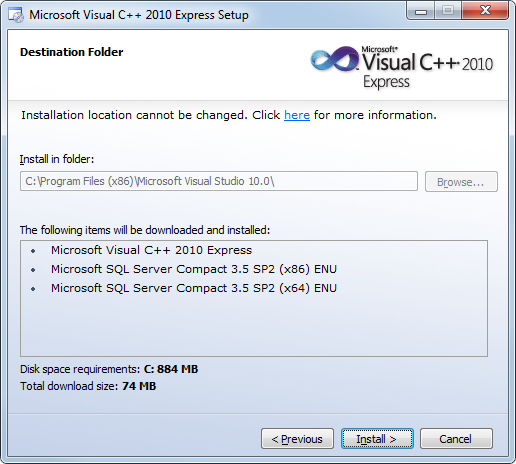
\includegraphics[scale=0.75]{figures/PNG/setup_vs_destination.png}
%	\caption{Visual C++ 2010 Express destination directory.}
%	\label{fig:setup_vs_destination}
%\end{figure}

	\item Wait for \emph{Visual C++} setup to finish downloading and installation. % (Figure~\ref{fig:setup_vs_install}).

%\begin{figure}[htbp]
%	\centering
%	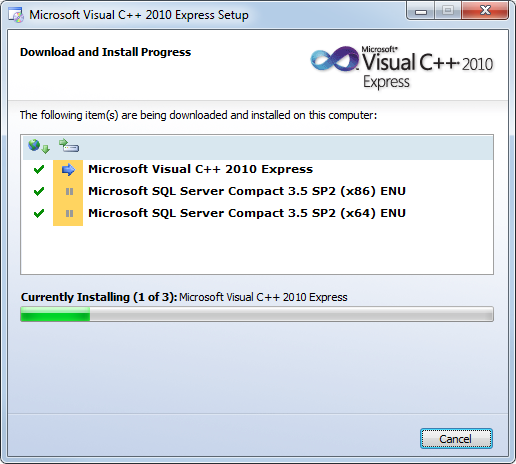
\includegraphics[scale=0.75]{figures/PNG/setup_vs_install.png}
%	\caption{Visual C++ 2010 Express download and install progress.}
%	\label{fig:setup_vs_install}
%\end{figure}

	\item After a few minutes, \emph{Visual C++} setup will report that the installation has finished. % (Figure~\ref{fig:setup_vs_success}).
		In some cases, a reboot may be required to use \emph{Visual C++}.

%\begin{figure}[htbp]
%	\centering
%	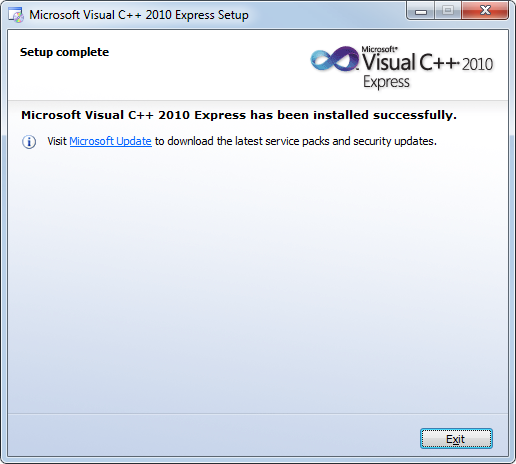
\includegraphics[scale=0.75]{figures/PNG/setup_vs_success.png}
%	\caption{Visual C++ 2010 Express setup complete.}
%	\label{fig:setup_vs_success}
%\end{figure}

\end{enumerate}

\clearpage
%
% Copyright (c) 2011-2012, fortiss GmbH.
% Licensed under the Apache License, Version 2.0.
% 
% Use, modification and distribution are subject to the terms specified
% in the accompanying license file LICENSE.txt located at the root directory
% of this software distribution. A copy is available at
% http://chromosome.fortiss.org/.
%
% This file is part of CHROMOSOME.
%
% $Id$
%
% Author:
%         Michael Geisinger <geisinger@fortiss.org>
%

\section{Installing CMake}
\label{appx:install_cmake}

Follow these steps to install CMake:

\begin{enumerate}
	\item Point your faviorite browser to \url{http://cmake.org/cmake/resources/software.html}
		and click on the link corresponding to the Windows installer
		(compare Figure~\ref{fig:setup_cmake_download}).

\begin{figure}[htbp]
	\centering
	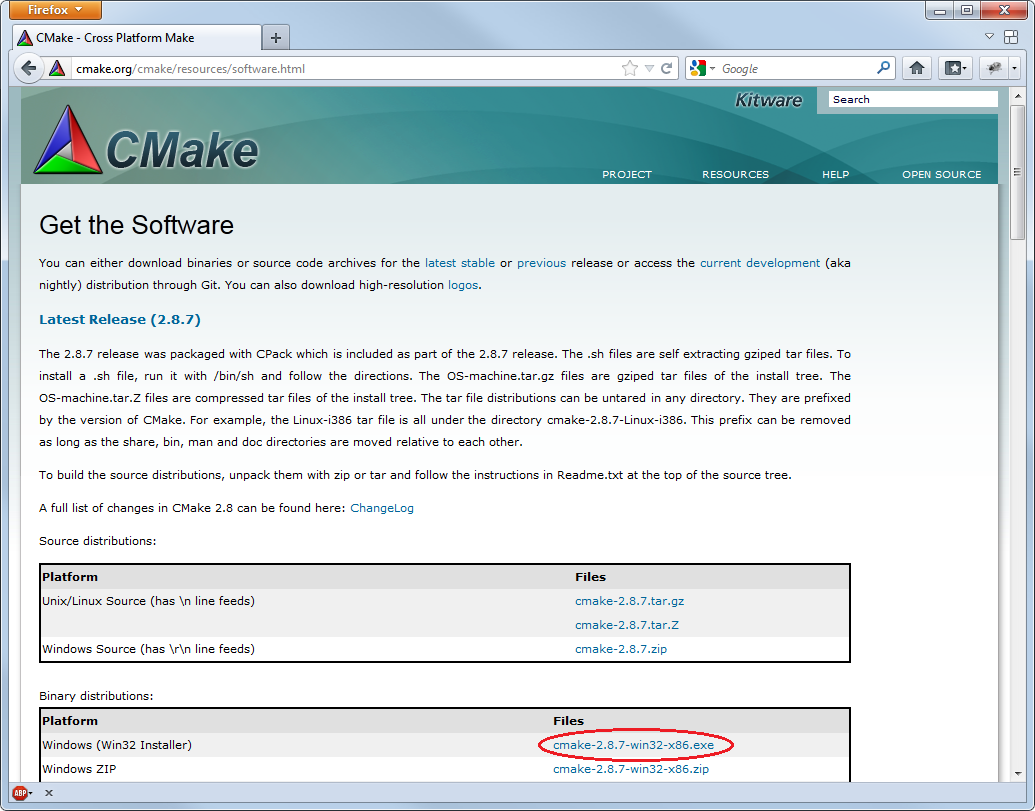
\includegraphics[scale=0.4]{figures/PNG/setup_cmake_download_edited.png}
	\caption{Selecting CMake for download, highlighted in red the download link.}
	\label{fig:setup_cmake_download}
\end{figure}

	\item After downloading the setup, launch it. Follow the instructions on the screen.
		When you get prompted whether to add CMake to the system PATH, you may choose to \emph{not} add it
		(compare Figure~\ref{fig:setup_cmake_path}).
		\xme does not require CMake to be on the system search path.

\begin{figure}[htbp]
	\centering
	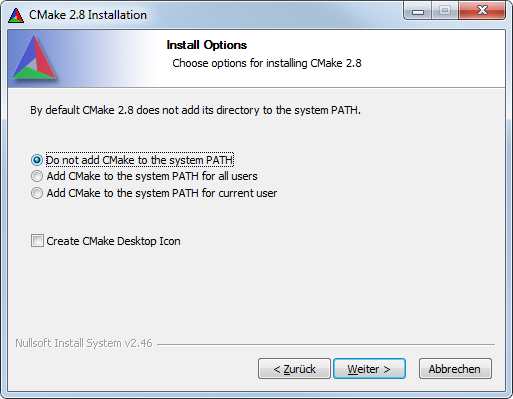
\includegraphics[scale=0.75]{figures/PNG/setup_cmake_path.png}
	\caption{CMake system PATH options.}
	\label{fig:setup_cmake_path}
\end{figure}

\end{enumerate}

\clearpage
%
% Copyright (c) 2011-2012, fortiss GmbH.
% Licensed under the Apache License, Version 2.0.
% 
% Use, modification and distribution are subject to the terms specified
% in the accompanying license file LICENSE.txt located at the root directory
% of this software distribution. A copy is available at
% http://chromosome.fortiss.org/.
%
% This file is part of CHROMOSOME.
%
% $Id$
%
% Author:
%         Michael Geisinger <geisinger@fortiss.org>
%

\section{\xme License}
\label{appx:license}

\lstset{basicstyle=\tt\footnotesize,language=,tabsize=4,escapechar=,emph=}
\lstinputlisting{../../../LICENSE.txt}


\end{document}
